\part{Applications of COLD}\label{part:applications}

\chapter{Optimising for properties of the state}\label{chap:6_Applications_fidelity}

\epigraph{In theory, theory and practice are the same. In practice, they are not.}{Unknown}

In Ch.~\ref{chap:4_COLD} we introduced \acrref{COLD}, a new method for speeding up adiabatic processes while suppressing non-adiabatic losses. In this chapter, we will investigate how such a method might perform for different adiabatic protocols in different physical systems via results from numerical simulations. 

There are a number of parameters that can be varied in each instance of applying COLD, including different ways to construct the control pulse (Sec.~\ref{sec:4.2_COLD_QOCT}), physical constraints placed on the system and the operator basis used for the \acrref{LCD}, among others. Furthermore, it is important to compare the effects of \acrref{COLD} against either of its two components: \acrref{LCD} and quantum optimal control, which have been implemented with the same goal as \acrref{COLD} in the past \cite{sels_minimizing_2017, glaser_training_2015, guery-odelin_shortcuts_2019}. We made the claim, in Ch.~\ref{chap:4_COLD}, that \acrref{COLD} should outperform either approach simply by construction and here we will demonstrate this in practice.

We will begin with an example of a two-spin annealing process in order to illustrate the \acrref{COLD} approach in detail, as well as the variational method for deriving an \acrref{LCD} pulse and constructing an optimal control pulse. We will then proceed to illustrate how \acrref{COLD} can be applied for a series of different example Hamiltonians and systems, starting with the Ising spin chain in Sec.~\ref{sec:5.2_Ising_chain}, then a case of population transfer in a synthetic lattice via an adiabatic rapid passage (\acrref{ARP}) protocol in Sec.~\ref{sec:5.3_synthetic} and finally in preparing maximally entangled states in a system of frustrated spins in Sec.~\ref{sec:6.4_ghz_states}. We will demonstrate how driving amplitude constraints affect the performance of \acrref{COLD} and other approaches in Sec.~\ref{sec:6.2.1_restricting_amps} and how different optimisation cost functions can inform the results in Sec.~\ref{sec:6.4.1_t3} where we will use entanglement as an optimisation metric instead of final state fidelity.

\section{Two-spin annealing}\label{sec:5.1_2spin_annealing}

To showcase and explore the use of \acrref{COLD} in a relatively simple setting we will consider a two spin quantum annealing problem with Hamiltonian
\begin{equation}\label{eq:two_spin_hamiltonian}
H_0(\hbb, \lambda) = J(\lambda) \sz_1 \sz_2 + Z(\lambda) ( \sz_{1} + \sz_{2}) +  X(\lambda) (\sx_{1} + \sx_{2}),
\end{equation}
where the operator subscripts denote the index of the spin on which they act, $H_0$ is parameterised by the functions $\hbb = \{J(\lambda), Z(\lambda), X(\lambda)\}$, with the $\lambda(t) = \frac{t}{\tau}$ term encoding the time-dependence and where $J(\lambda) = -2J_0$ and $z(\lambda) = -h_0$ are constant functions. For this example we use
\begin{equation}\label{eq:lambda_func1}
X(\lambda) = 2 h_0 \sin^2\left(\frac{\pi}{2} \sin^2 \left( \frac{\pi}{2} \lambda \right) \right),
\end{equation}
where we note that since $\lambda(0) = 0$ and $\lambda(\tau) = 1$, the transverse field is tuned from $0$ to $2h_0$ as $t$ goes from $0$ to $\tau$. We consider the case where $J_0/h_0 = 0.5$, meaning that the initial ground state of the system is in the $\ket{\uparrow \uparrow}$ state and the ground state at $t = \tau$ should be a superposition of all the symmetric states.

As per the discussion in in Sec.~\ref{sec:2.4.1_LCD}, since $H_0$ is a real-valued Hamiltonian, the single-spin LCD operators should be fully imaginary and thus given by the following ansatz for the adiabatic gauge potential:
\begin{equation}\label{eq:LCD1st}
\approxAGP^{(1)}(\lambda, \hbb) = \alpha(\lambda, \hbb) (\sy_1 + \sy_2),
\end{equation}
which we will indicate as `first-order' or \acrref{FO} \acrref{LCD}, referring to the fact that these are the most local spin operators and denoting this fact with the superscript $(1)$. In this case, we expect the \acrref{LCD} pulse to be the same for both $\sy_1$ and $\sy_2$ due to the symmetry of the Hamiltonian, hence only requiring one coefficient $\alpha$ for both operators. In future sections where this is not the case, we will instead differentiate between global and local \acrref{LCD} pulses, where unique pulses may be required for each separate operator, but due to physical constraints we approximate them with a single coefficient.

Using the methods described in \cite{sels_minimizing_2017} and summarised in Sec.~\ref{sec:2.4.1_LCD}, we can determine the form of the coefficient $\alpha$ using a variational approach, which I will set out in detail here to illustrate the method. For the given $H_0$, and $\approxAGP$, the first step is to find the operator $G_{\lambda}$ from Eq.~\ref{eq:G_operator}:
\begin{equation}
    \begin{aligned}
        G_{\lambda}(\approxAGP^{(1)}, H_0) &= \dlambda H_0 + \frac{i}{\hbar} \comm{\approxAGP^{(1)}}{H_0} \\
        &= \dlambda {X} (\sx_{1} + \sx_{2}) - 2 \alpha J (\sx_1\sz_2 + \sz_1\sx_2) - 2 \alpha Z (\sx_{1} + \sx_{2}) \\
        &+ 2 \alpha X (\sz_{1} + \sz_{2}),
    \end{aligned}
\end{equation}
where the $\lambda$-dependence is omitted and the only non-constant function is $X(\lambda)$, making it the only non-zerp contribution to $\dlambda H_0$. We then obtain the action from Eq.~\eqref{eq:agp_action} defined as $\mathcal{S} = \Tr[G^2_{\lambda}]$:
\begin{equation}
    \frac{1}{8} \Tr[G^2_{\lambda}] = 4 \alpha^2 X^2 + (\dlambda X - 2 \alpha Z)^2 + 4 \alpha^2 J^2,
\end{equation}
which can be minimised with respect to the coefficient $\alpha$ in order to find the \acrref{LCD} pulse:
\begin{equation}
    \begin{aligned}
        \frac{\partial \mathcal{S}}{\partial \alpha} &= 8X^2\alpha - 4Z(\dlambda X - 2 \alpha Z) + 8 J^2 \alpha = 0 \\
        & \Rightarrow \alpha = \frac{1}{2} \frac{Z \dlambda X}{X^2 + Z^2 + J^2},
    \end{aligned}
\end{equation}
where we find, as expected, that the \acrref{LCD} pulse is a function of $\lambda$ and the Hamiltonian coefficients $\hbb$ (and their derivatives with respect to $\lambda$). For completeness, the full \acrref{LCD} Hamiltonian, recalling Eq.~\eqref{eq:CD_Hamiltonian}, then reads:
\begin{equation}\label{eq:FO_LCD_H}
    \begin{aligned}
        H_{\rm LCD}(\hbb, \lambda) &= H_0(\hbb, \lambda) + \dotlambda \alpha(\hbb, \lambda) (\sy_{1} + \sy_{2}),
    \end{aligned}
\end{equation}
where the counterdiabatic pulse is simply the (approximate) \acrref{AGP} scaled by the rate of change in the time-dependent parameter $\lambda$.

We can do the same as above for the next most local, two-spin operators, which we will refer to as `second-order' or \acrref{SO} \acrref{LCD}. They too should be imaginary and, due to the Hamiltonian symmetry, can be cast into two groups with two different \acrref{LCD} coefficients $\gamma$ and $\zeta$:
\begin{equation}\label{eq:twospin_so_lcd}
        \approxAGP^{(2)}(\hbb, \lambda) = \gamma(\hbb, \lambda) (\sx_1 \sy_2 + \sy_1 \sx_2) + \zeta(\hbb, \lambda) (\sz_1 \sy_2 + \sy_1 \sz_2).
\end{equation}
These can be solved for in a similar vein to the method for $\alpha$, although in this case the minimisation of $\mathcal{S}(\approxAGP^{(2)})$ will happen separately for both $\gamma$ and $\zeta$, giving a coupled set of equations, which can be solved numerically. Since the whole system is only made up of two spins, the two orders of \acrref{LCD} ansatz are enough to characterise the \acrref{AGP} fully as they contain all completely imaginary orthogonal operators in the Pauli basis. Thus, solving the coupled set of equations
\begin{equation}\label{eq:two_spin_coupled_eqs}
        \begin{pmatrix}
        2(X^2 + Z^2 + J^2) & - 2JX & 4JZ \\ 
        -XJ & X^2 + 4Z^2 & -3XZ \\ 
        4JZ & -6ZX & 2J^2 + 2Z^2 + 8X^2
        \end{pmatrix} 
        \begin{pmatrix}
            \alpha \\
            \gamma \\
            \zeta
        \end{pmatrix} = 
        \begin{pmatrix}
            Z \dlambda X \\
            0 \\
            J \dlambda X
        \end{pmatrix}
\end{equation}
for the coefficients $\alpha$, $\gamma$ and $\zeta$ should give the exact \acrref{AGP} operator 
\begin{equation}\label{eq:two_spin_exact_AGP}
    \AGP{\lambda}(\hbb, \lambda) = \alpha(\hbb, \lambda) (\sy_1 + \sy_2) + \gamma(\hbb, \lambda) (\sx_1 \sy_2 + \sy_1 \sx_2) + \zeta(\hbb, \lambda) (\sz_1 \sy_2 + \sy_1 \sz_2)
\end{equation}
for the Hamiltonian $H_0(\hbb, \lambda)$ given any $\hbb$ and $\lambda$. 

\begin{figure}[t]
    \centering
    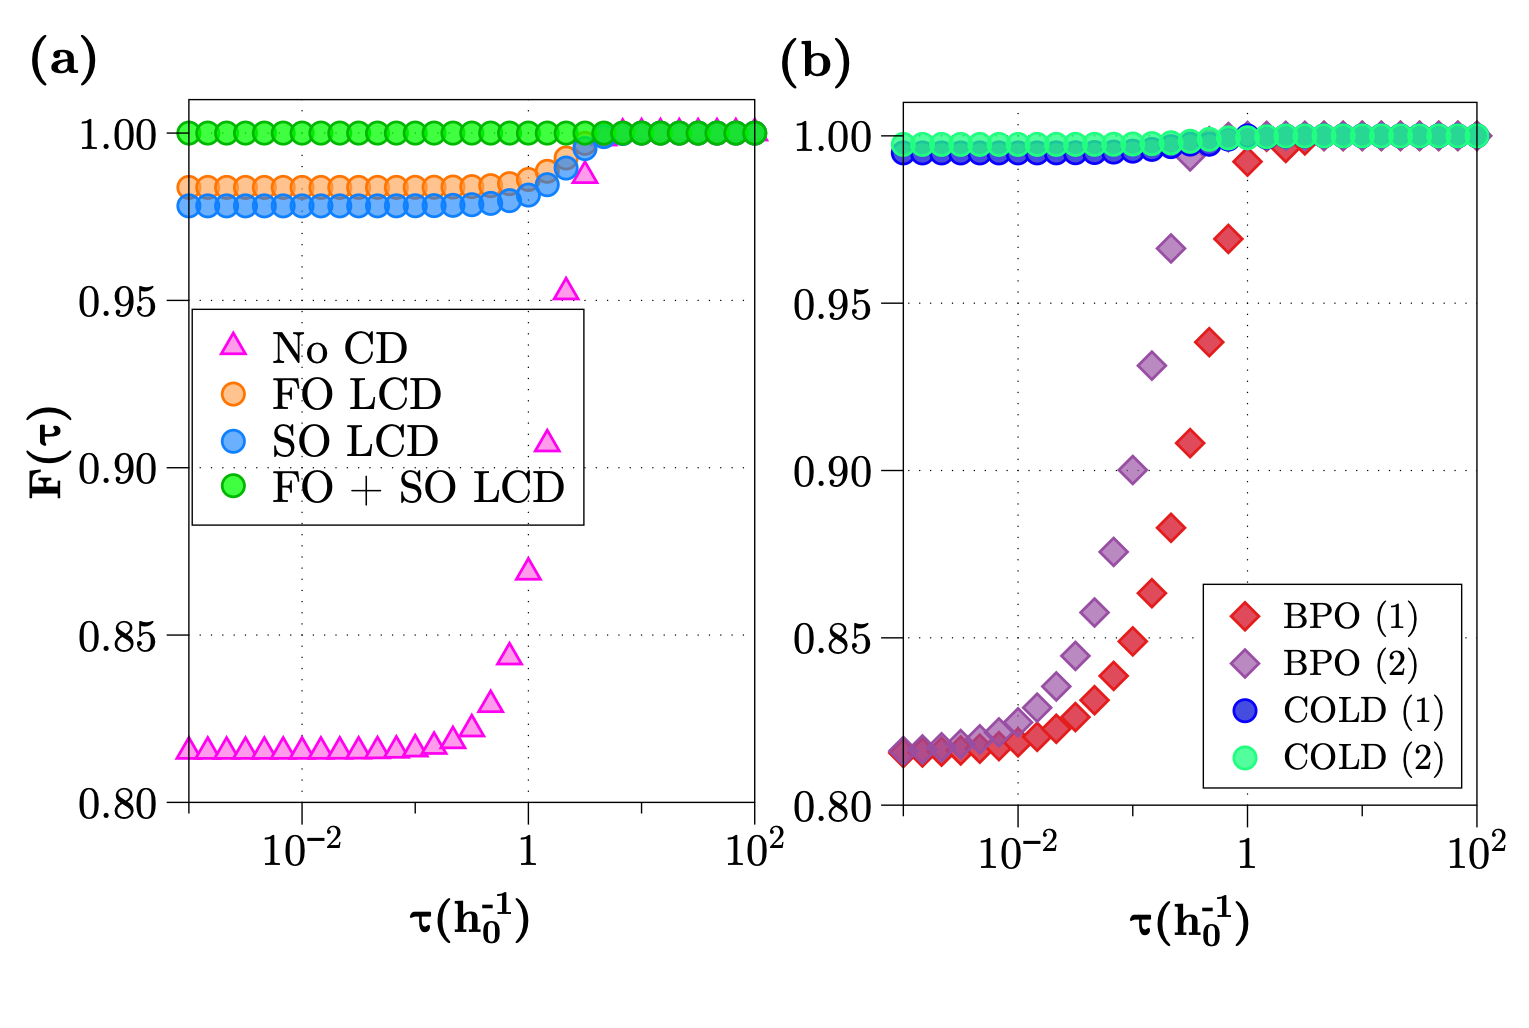
\includegraphics[width=0.8\linewidth]{images_v1/twospins_fidelities.png} \caption[COLD applied to two-spin annealing]{Optimisation of the annealing protocol for two spin Hamiltonian given by Eq.~\eqref{eq:two_spin_hamiltonian} and with parameters as described in the main text.  (a) Final fidelities of the annealing protocol with triangles (pink) representing the case where no \acrref{CD} is applied and circles showing the case of \acrref{FO} \acrref{LCD} (orange), \acrref{SO} \acrref{LCD} (blue) as well as the combination of \acrref{FO} and \acrref{SO} \acrref{LCD} (green). (b) Final fidelities achieved when using the optimal control method \acrref{BPO} ($N_k = 1$: red diamonds, $N_k = 2$: purple diamonds) and \acrref{COLD} ($N_k = 1$: blue circles, $N_k = 2$: aquamarine circles) with \acrref{FO} \acrref{LCD} operators as described in the text.}\label{fig:twospin_fidelities}
\end{figure}

The different approaches are demonstrated in Fig~\ref{fig:twospin_fidelities}(a) via numerical simulations of the system evolution for different total evolution times $\tau (h_0^{-1})$. We compare the final evolved state $\ket{\psi(\tau)}$ of the system with the ground state of $H_0(\lambda = 1)$ denoted by $\ket{\psi_{GS}}$ by computing their fidelity:
\begin{equation}
    F(\tau) = \left|\braket{\psi_{GS}}{\psi(\tau)}\right|^2.
\end{equation}
The results are computed for the case where only the bare Hamiltonian $H_0(\hbb, \lambda)$ from Eq.~\ref{eq:two_spin_hamiltonian} drives the system and they are then compared to \acrref{FO} \acrref{LCD} (Eq.~\eqref{eq:FO_LCD_H}), \acrref{SO} \acrref{LCD} (the solution to Eq.~\eqref{eq:two_spin_coupled_eqs} with $\alpha$ set to $0$) and the exact counterdiabatic drive (Eq.~\eqref{eq:two_spin_exact_AGP}). The results show that at fast evolution times ($\tau < 1 h_0^{-1}$) when no counterdiabatic drive is applied the final state remains far from the ground state of $H_0(\lambda = 1)$ and only begins to approach the target as the evolution time is increased, exactly as one might expect given the adiabatic condition (Sec.~\ref{sec:2.1.2_adiabatic_condition}). In the case of both \acrref{FO} and \acrref{SO} \acrref{LCD}, however, the system approaches the desired ground state with close to unit fidelity even at very short driving times several orders of magnitude faster. As expected, when the exact \acrref{CD} is applied including all single- and two-spin imaginary operators, the system reaches the desired state with unit fidelity at arbitrarily short driving times, as in the rotating spin example we discussed in Ch.~\ref{chap:2_adiabaticity} and Appendix~\ref{app:rotating_spin_hamiltonian}.

At this point all we have done is to implement the \acrref{LCD} method for a simple example where the exact \acrref{CD} can be easily derived. This was done primarily to illustrate how the \acrref{LCD} pulse is constructed and how it can be used to significantly speed up system evolution while driving it close to the target state by suppressing a large proportion of non-adiabatic losses. With these components explored in depth, we can now finally introduce \acrref{COLD} in a practical setting.

As the goal of \acrref{COLD} is to improve \acrref{LCD} in restricted settings, the most natural approach to demonstrate it in a simple example like this is to take the \acrref{FO} \acrref{LCD} ansatz as a fixed approximation for the counterdiabatic drive and to ignore \acrref{SO} terms. This is a realistic scenario, as even two-spin operators like those found in the \acrref{SO} \acrref{LCD} anstaz of Eq.~\eqref{eq:twospin_so_lcd} are generally difficult to engineer in physical systems and thus even in this simple case it is unlikely that the exact \acrref{CD} pulse could be implemented, though its functional form is known.

Revisiting Ch.~\ref{chap:4_COLD}, we find that the first step of \acrref{COLD} is to construct a control pulse for the Hamiltonian. Ideally, this is something that can be easily controlled in an experimental setting and for the given $H_0$, we can imagine introducing a $\lambda$-dependent control for the coupling, transverse or longitudinal fields. For simplicity and pedagogy, we can introduce a `bare' pulse (Sec.~\ref{sec:4.2_COLD_QOCT}) control component to the Hamiltonian which drives the $(\sz_1 + \sz_2)$ operators and obeys the constraint of being $0$ at the beginning and end of the driving time. This gives a control Hamiltonian:
\begin{equation}\label{eq:COLD_twospin_controlH}
    \begin{aligned}
        H_\beta(\betabb, \hbb, \lambda) &= H_0(\hbb, \lambda) + \sum_{k=1}^{N_k} \beta_k(\lambda) (\sz_{1} + \sz_{2}) \\
        &= H_0(\hbb, \lambda) + \sum_{k=1}^{N_k} c_k \sin (\pi k \lambda) (\sz_{1} + \sz_{2}),
    \end{aligned}
\end{equation}
where $\beta_k(\lambda) \in \betabb$, $\beta_k(\lambda) = c_k \sin (\pi k \lambda)$, the value $N_k$ denotes the total number of control functions and the parameters $c_k$ can be optimised using a numerical optimal control method introduced in Sec.~\ref{sec:3.1.3_numerical_optimisation}. In this case, we will implement Powell optimisation (Sec.~\ref{sec:3.1.3.2_Powell}) as it is an efficient, gradient-free method that heuristically appears to avoid local minima in the cost function space better than Nelder-Mead (Sec.~\ref{sec:3.1.3.1_Nelder_Mead}), although both can be used given the relatively simple control problem at hand. 

Since the control Hamiltonian includes additional non-trivial $\lambda$-dependent components that $H_0$ did not, we need to re-derive the updated \acrref{FO} \acrref{LCD} pulse for the control Hamiltonian $H_{\beta}$, which is not particularly difficult if we follow the earlier recipe:
\begin{equation}\label{eq:twospin_alpha_COLD}
    \alpha(\betabb, \hbb, \lambda) = \frac{1}{2} \frac{(Z + f_{\rm opt}^{N_k}) \dlambda X - (\dlambda f_{\rm opt}^{N_k}) X}{(Z + f_{\rm opt}^{N_k})^2 + X^2 + J^2},
\end{equation}
where $f_{\rm opt}^{N_k} = \sum_{k=1}^{N_k} \beta_k$ is the full control pulse constructed out of the $N_k$ components. The total \acrref{COLD} Hamiltonian with \acrref{FO} \acrref{LCD} is then:
\begin{equation}\label{eq:twospin_COLD_Ham}
    H_{\rm COLD}(\betabb, \hbb, \lambda) = H_0(\hbb, \lambda) + f_{\rm opt}^{N_k}(\betabb, \lambda)(\sz_1 + \sz_2) + \dotlambda \alpha(\betabb, \hbb, \lambda)(\sy_1 + \sy_2).
\end{equation}

All that remains is to optimise the parameters $c_k$ with Powell's optimisation algorithm. As our goal is to drive the system to the ground state of $H_0(\lambda = 1)$, we can implement the fidelity cost function from Eq.~\eqref{eq:costfunc_fidelity} as a metric for the optimisation. Fig.~\ref{fig:twospin_fidelities}(b) shows the results of numerical simulations in the same regime as for the optimisation-free case, comparing evolution under the optimal control Hamiltonian from Eq.~\eqref{eq:COLD_twospin_controlH}, an approach we call `Bare Powell Optimisation' or \acrref{BPO} and the \acrref{COLD} Hamiltonian (Eq.~\eqref{eq:twospin_COLD_Ham} with a \acrref{FO} \acrref{LCD} pulse included. Even for a single optimisable parameter, \acrref{COLD} achieves $\sim 99.5\%$ fidelity at arbitrarily short times, while \acrref{BPO} remains stuck below $\sim 85\%$ until $\tau \sim 0.1h_0^{-1}$. Both approaches show some improvement with an added control parameter ($N_k = 2$), with the \acrref{COLD} result starting at $\sim 99.8\%$ fidelity even at short times. Neither approach, however, shows any noticeable improvement when adding more control parameters beyond this. 

Before moving on to the next section, I want to note that this example is very simple and largely pedagogical. It may be possible to improve the results of both \acrref{BPO} and \acrref{COLD} with more sophisticated optimal control techniques, but it shows that even in the simplest case, \acrref{COLD} is a powerful method. If reliable access to the operators making up the exact \acrref{CD} is available, then it is better to implement \acrref{CD} rather than attempting optimal control. However, as this is almost never the case given the complexity and non-locality of the exact \acrref{AGP}, \acrref{COLD} is the best way to make the most out of the limited counterdiabatic capacity available.

\section{Ising chain}\label{sec:5.2_Ising_chain}

A more complex and widely studied example system that we can apply \acrref{COLD} to is the one-dimensional Ising spin chain for $N$ spins in the presence of a transverse and longitudinal field. The Ising model is a fundamental model in quantum mechanics and its ground states can be used to encode solutions to many combinatorics problems \cite{mohseni_ising_2022, ebadi_quantum_2022, pichler_quantum_2018}. As such, studying annealing protocols for Ising Hamiltonians with arbitrary connectivity is of particular interest. While in this section we will look only at the restricted case of the Ising chain, in Appendix~\ref{app:arbitrary_ising_derivation} I derive the coupled equations for \acrref{FO} and \acrref{SO} \acrref{LCD} coefficients for a model with arbitrary $\sz\sz$ connectivity between the spins.

The Ising chain is described by the Hamiltonian
\begin{equation}\label{eq:ising_chain_hamiltonian}
    H_0(\hbb,\lambda) = J(\lambda) \sum_{j}^{N-1} \sz_j \sz_{j+1} + Z_0\sum_j^N \sz_j + \lambda X_f \sum_j^N \sx_j,
\end{equation}
where once again $\lambda(t) = t/\tau$, $\hbb = \{ J(\lambda), Z(\lambda), X(\lambda) \}$ with constant functions $J(\lambda) = -J_0$, $Z(\lambda) = Z_0$ and
\begin{equation}
    X(\lambda) = X_0 \sin^2\left(\frac{\pi}{2} \sin^2 \left( \frac{\pi}{2} \lambda \right) \right).
\end{equation}
In this section, all results are obtained using $J_0 = 1$, $Z_0 = 0.02J_0$ and $X_0 = 10J_0$.

Many of the steps in this section will be rehashed from the two spin example as the approach is very similar. In this case, we will only focus on the \acrref{FO} \acrref{LCD} terms, which are the single-spin $\sy$ operators applied to each spin in the chain, in the same vein as in the two spin example  of Eq.~\ref{eq:LCD1st} due to the Hamiltonian being real:
\begin{equation}\label{eq:ising_fo_agp}
    \approxAGP^{(1)}(\hbb, \lambda) = \alpha(\hbb, \lambda) \sum_{j}^N\sy_j,
\end{equation}
where using the variational \acrref{LCD} approach we find that 
\begin{equation}
    \alpha = \frac{1}{2} \frac{Z \dlambda X}{X^2 + Z^2 + 2(1 - 1/N)J^2},
\end{equation}
with the $N$-dependent factor in the denominator is a consequence of the edge effects of the chain which disappear in the case of a ring. 

\begin{figure}[t]
    \centering
    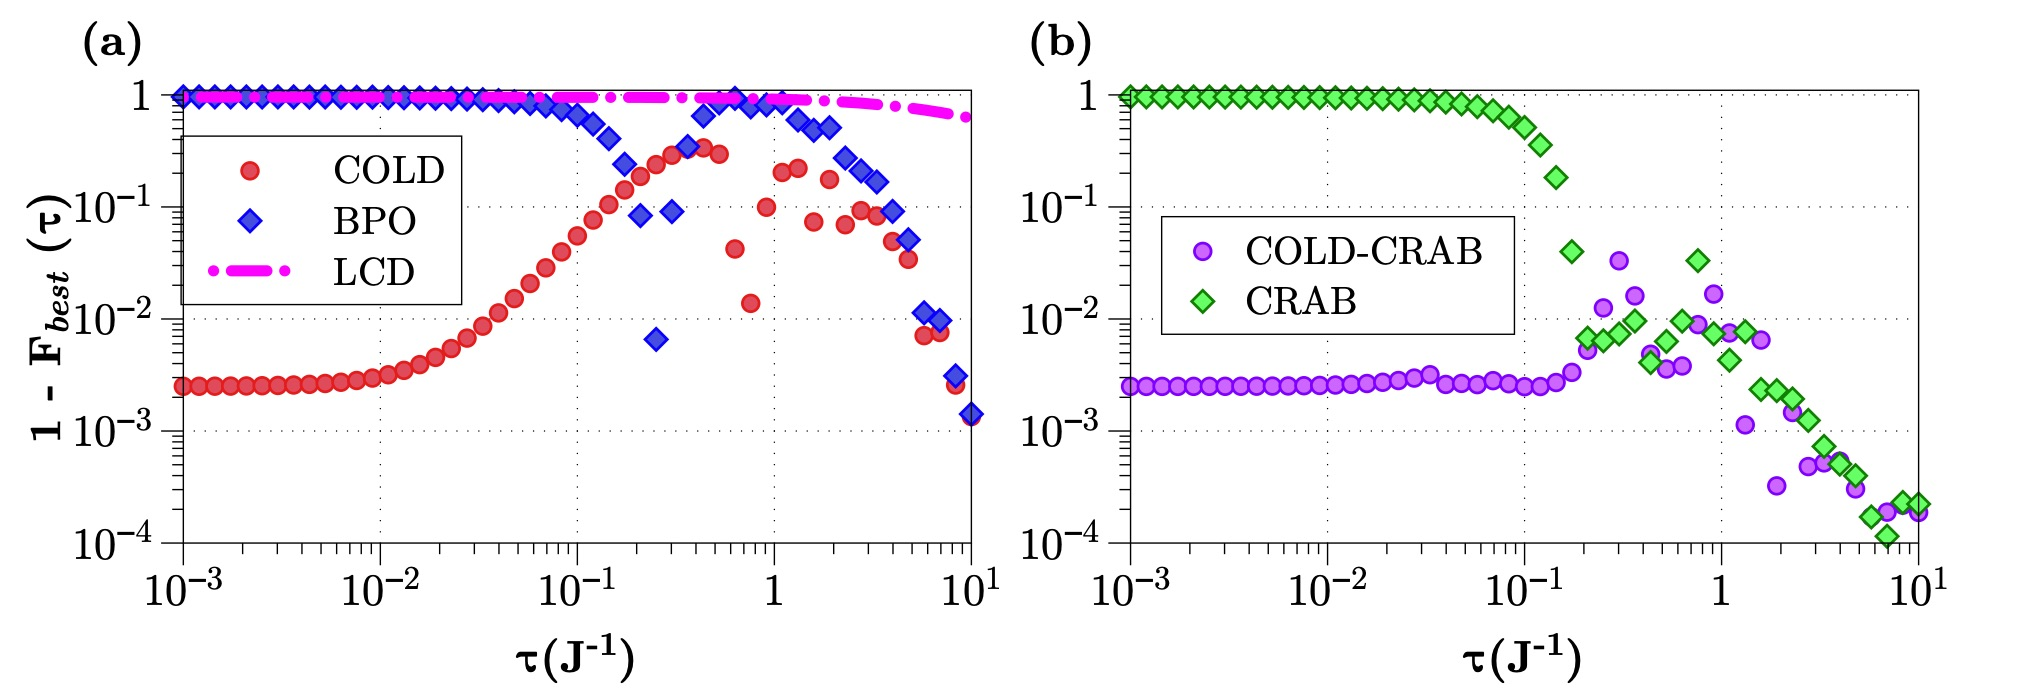
\includegraphics[width=\linewidth]{images_v1/IsingUnconstrained.jpg} \caption[Applying COLD and COLD-CRAB to the Ising chain for 5 spins without constraints on the driving amplitudes.]{Final state fidelities for the Ising spin chain example described in the text for $N=5$ spins. In (a) we plot the best $(1 - F(\tau))$ obtained from 500 optimisations for different evolution times $\tau$ in the case where only \acrref{FO} \acrref{LCD} is applied (pink dash-dot line), as well as \acrref{BPO} (Eq.~\eqref{eq:ising_chain_BPO_H}, blue diamonds) and \acrref{COLD} with \acrref{FO} \acrref{LCD} (red circles) with a bare pulse control as described in the text. (b) shows implementations of \acrref{CRAB} and \acrref{COLD}-\acrref{CRAB}, with the best result again chosen from 500 optimisations, each with a different randomised frequencies in the trigonometric basis as described in the text. All control pulses use $N_k = 1$ optimisable parameter. Figure reproduced from \cite{cepaite_cold_2023}.} \label{fig:ising_unconstrained}
\end{figure}

In order to implement \acrref{COLD} we need to once again construct a control pulse. In this case, we will start with a similar naive bare pulse as in the two spin case from the previous section
\begin{equation}\label{eq:ising_chain_BPO_H}
    \begin{aligned}
        H_{\beta}(\betabb, \hbb, \lambda) &= H_0(\hbb, \lambda) + \sum_k^{N_k} \beta_k(\lambda) \sum_j \sz_j \\
        &= H_0(\hbb, \lambda) + \sum_k^{N_k} c_k \sin(\omega_k \lambda) \sum_j \sz_j,
    \end{aligned}
\end{equation}
with $\omega_k = 2\pi k$ the $k$th principal frequency. In the case where no \acrref{LCD} is added to this Hamiltonian, we will again refer to the method as \acrref{BPO} as the numerical optimisation is carried out using Powell's method.

To construct the \acrref{COLD} Hamiltonian, the only additional step is to include the \acrref{LCD} pulse which we will restrict to single-spin terms as in Eq.~\eqref{eq:ising_fo_agp}:
\begin{equation}
    H_{\rm COLD}(\betabb, \hbb, \lambda) = H_0(\hbb, \lambda) + f_{\rm opt}^{N_k}(\betabb, \lambda)\sum_j \sz_j + \dotlambda \alpha(\betabb, \hbb, \lambda)\sum_j \sy_j,
\end{equation}
where again $f_{\rm opt}^{N_k} = \sum_k^{N_k} \beta_k(\lambda)$ represents the full control pulse made up of $N_k$ functions. 

As well as the bare pulse, however, in this case we will also implement the \acrref{CRAB} algorithm which was first introduced in Sec.~\ref{sec:3.3.1_CRAB} and compare it to the naive approach. The \acrref{COLD} algorithm with a \acrref{CRAB}-type pulse is thus referred to as \acrref{COLD}-\acrref{CRAB}. In our case, the inclusion of \acrref{CRAB} simply necessitates adding a randomised component to the naive basis functions $\beta_k(\lambda)$. Namely, the pulse $f_{\rm opt}^{N_k}$ is replaced by $f_{\rm CRAB}^{N_k}$ where the principal frequencies $k$ are modified as $k \rightarrow k(1+r_k)$, with $r_k$ drawn from a uniform random distribution $r_k \in [-0.5,0.5]$ such that:
\begin{equation}\label{eq:ising_crab_pulse}
    f_{\rm CRAB}^{N_k} = \sum_k^{N_k} c_k \sin(2 \pi k(1+r_k)\lambda).
\end{equation}
Since each optimisation instance for the \acrref{CRAB} algorithm will implement a slightly different pulse for the same number of control parameters owing to the randomised component, it is liable to lead to cost functions that have both better and worse minima than those of the naive pulse, meaning that the optimisation needs to be carried out many times in order to be sure of exploring as much of the solution space as possible. This added complexity is, as already discussed in Sec.~\ref{sec:3.3.1_CRAB}, what generally makes \acrref{CRAB} a better approach in terms of results obtained and a more difficult one due to the computational overhead required for the optimisation.  

In Fig.~\ref{fig:ising_unconstrained}(a) we plot the results for the \acrref{FO} \acrref{LCD}, \acrref{BPO} and \acrref{COLD} for $N=5$ spins, noting that unlike in the two spin case, the \acrref{LCD} approach for this set of operators no longer shows a significant speed up, with final state fidelities remaining low even at long times. In fact, for all plotted times, it shows barely a $1\%$ improvement in fidelity over the bare Hamiltonian, which is not plotted as it would not be visible owing to it almost overlapping with the \acrref{LCD} line. The \acrref{BPO} approach, on the other hand, appears to perform better at longer times with a sharp increase in fidelity around what is likely a natural timescale for the system, where it dips below the \acrref{COLD}. The \acrref{COLD} approach, as before, performs really well at short driving times, where it is orders of magnitude better than either \acrref{LCD} or \acrref{BPO}. At longer times, this advantage wanes whether due to the optimisation process as multiple minima emerge in the cost function landscape or due to the fact that the local non-adiabatic effects are no longer the main source of losses. 

Fig.~\ref{fig:ising_unconstrained}(b) shows the results when using \acrref{CRAB} as well as \acrref{COLD}-\acrref{CRAB} in the same setting, with both performing far better at longer times than their naive \acrref{BPO} and \acrref{COLD} counterparts in plot (a) respectively, but remaining at similar levels of performance at short times, likely due to something more fundamental like the geometric speed limit \cite{bukov_geometric_2019}. This is definitely an argument for using something more sophisticated like \acrref{COLD}-\acrref{CRAB} as a general rule, as long as the computational resources are available for many and/or parallel optimisation instances.

While in Fig.~\ref{fig:ising_unconstrained} we only explore one optimisable parameter $N_k = 1$ and a system size of $N=5$ spins, the resulting advantage of \acrref{COLD} over bare optimisation scales with system size and we find that, at least in the case of the naive pulse, increasing the number of parameters does not seem to make too much of a difference. These results and more discussion can be found in Appendix~\ref{app:ising}.

\subsection{Restricting the driving amplitudes}\label{sec:6.2.1_restricting_amps}

While it is all well and good to talk about practical protocols implementing only local \acrref{LCD} operators with control drives that can be accessed by real experiments, one thing that we have so far failed to mention and which is not hard to observe from the form of the \acrref{CD} drive in Eq.~\ref{eq:CD_Hamiltonian}, is that the amount of power required for the counterdiabatic pulse at short times scales with the speed of the changing Hamiltonian due to the $\dotlambda$ coefficient. This means that while both \acrref{LCD} and \acrref{COLD} may lead to really high final state fidelities at very short driving times, they might also do this at the cost of impossibly high power requirements for the drives that implement the counterdiabatic component in either approach.

We find, (details in Fig.~\ref{fig:ising_maxamp} in Appendix~\ref{app:ising}), that this is indeed what happens in the Ising chain case: as the total time of the evolution is reduced, the maximum amplitude reached by the \acrref{LCD} pulse increases, leading to two orders of magnitude in difference between the power requirements at $\tau = 10^{-3}J_0^{-1}$ and $\tau = 10^{-1}J_0^{-1}$. As one of the goals of \acrref{COLD} as a method is to be practically implementable, this result is inherently counterproductive.

\begin{figure}[t]
    \centering
    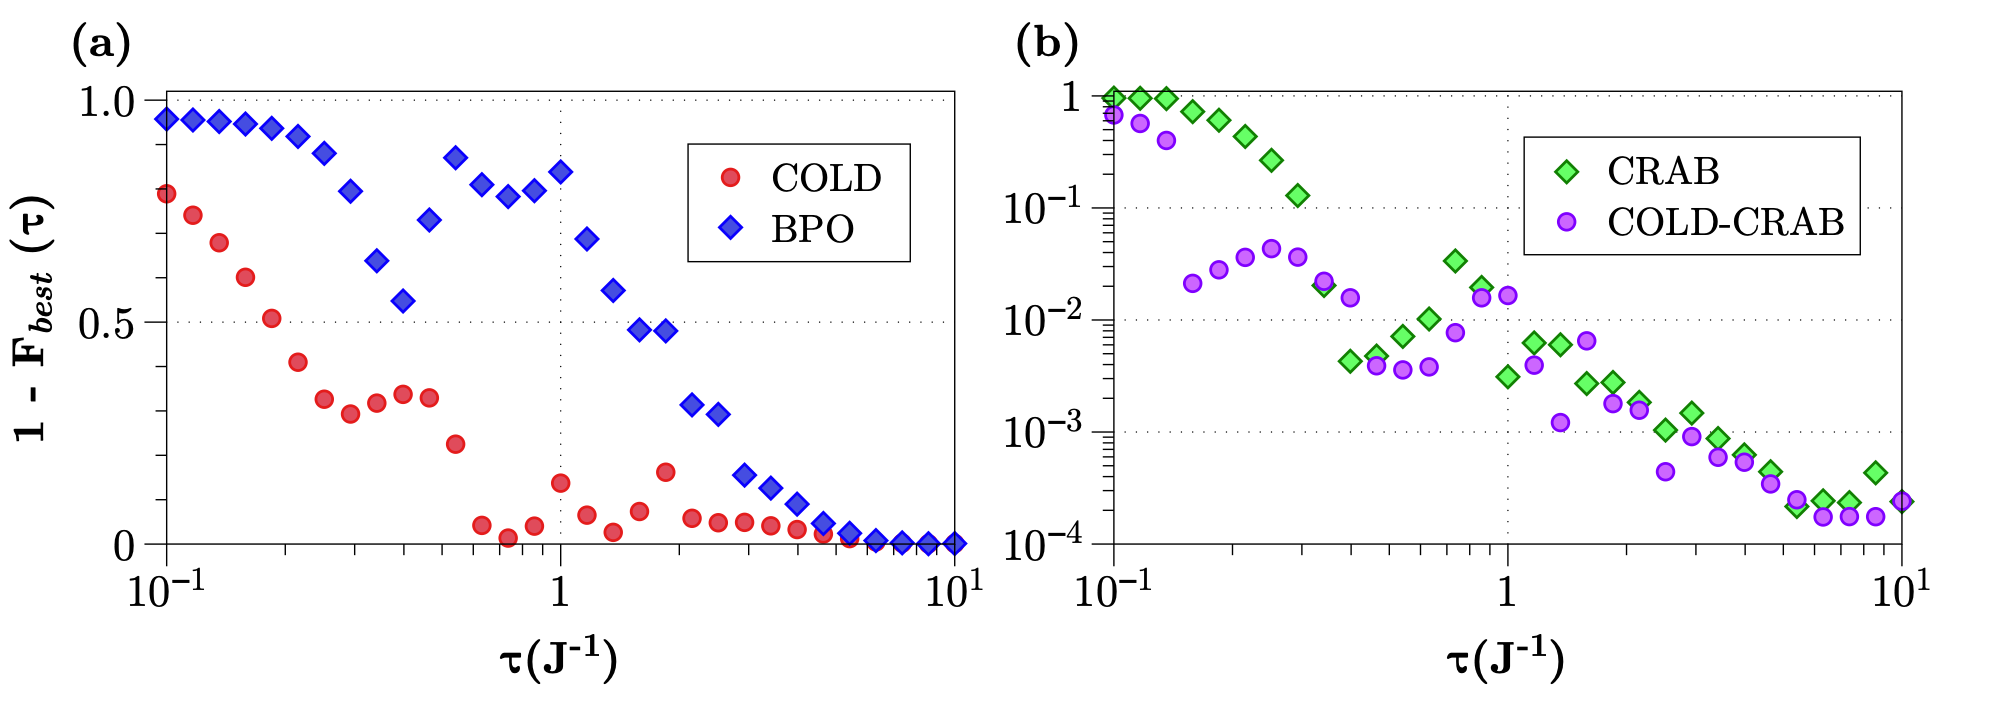
\includegraphics[width=\linewidth]{images_v1/IsingcConstrained.png} \caption[Applying COLD and COLD-CRAB to the Ising chain for 5 spins with constrained driving amplitudes.]{Optimisation of the constrained annealing protocol for the Ising model for $N=5$ spins with a maximum amplitude limit on each term in the Hamiltonian of Eq.~\eqref{eq:ising_chain_hamiltonian} of $X_0 = 10J_0$. (a) shows a comparison between BPO (blue diamonds). In (b) the comparison is between CRAB (green diamonds) and COLD-CRAB (purple circles). The plotted best results are obtained from 200 optimisations for each method. Figure reproduced from \cite{cepaite_cold_2023}.}\label{fig:ising_constrained}
\end{figure}

In order to solve this issue, we can include penalty terms in the cost function used to optimise the pulses for all of the different approaches: \acrref{BPO}, \acrref{COLD}, \acrref{CRAB} and \acrref{COLD}-\acrref{CRAB}. These penalty terms behave as constraints on the behaviour of the optimised pulse, and they may also include constraints on the \acrref{LCD} pulse that is included in \acrref{COLD}. If we take our original fidelity cost function from Eq.~\eqref{eq:costfunc_fidelity}, we can modify it by including terms that are conditioned on the maximum amplitude of a given pulse:
\begin{equation}
    C_F^{\rm const}(\hbb, \betabb, \lambda) = 1 - F(\hbb, \betabb, \lambda) + \sum_m \Lambda_m(\hbb, \betabb, \lambda),
\end{equation}
where $\Lambda_m(\hbb, \betabb, \lambda) = 0$ if the $m^{\rm th}$ constraint is satisfied and $\Lambda_m(\hbb, \betabb, \lambda) \gg \min(1 - F(\hbb, \betabb, \lambda))$ otherwise. We can implement such constraints for all of the driving amplitudes for all of the coefficients of each Hamiltonian, \@e.g.~$\alpha$, $f_{\rm opt}^{N_k}$ and $f_{\rm CRAB}^{N_k}$. In Fig.~\ref{fig:ising_constrained}, this is done for the case where any of the drives exceeds the maximum amplitude of any of the bare Hamiltonian $H_0$ coefficients, which in our case if when $X(\lambda = 1) = X_0 = 10J_0$. We find that, while the resulting fidelities are greatly reduced in the \acrref{BPO} and \acrref{COLD} cases, the \acrref{COLD} approach outperforms the plain optimal control method. The far better results are obtained using \acrref{CRAB} and \acrref{COLD}-\acrref{CRAB}, which require far more computational resources but, as expected, allow a lot more flexibility within the constraints to obtain good final state fidelities. 

The results presented here are supplemented further in Ch.~\ref{chap:7_higher_order_agp}, where we investigate how to use the ideas from Ch.~\ref{chap:5_cd_as_costfunc} in order to implement \acrref{CD}-based cost functions to optimise \acrref{COLD} and \acrref{BPO} for the Ising spin chain. Additional plots for different system sizes and information on the variances between result outcomes in different optimisation isntances are presented in Appendix~\ref{app:ising}.

\section{Transport in a synthetic lattice}\label{sec:5.3_synthetic}

Let us turn out sights to a completely different type of system for a moment and explore how \acrref{COLD} might perform. The efficient transfer of states between opposite ends of a lattice is an important protocol that could have future applications in the settings of quantum computation and simulation due to its promise of efficient transport of information \cite{lang_topological_2017}. This objective is often tackled in the setting of ultracold atoms in optical lattices. While the problem can be tuned to be a single-particle system and the analytical solutions of the corresponding instantaneous Schr\"odinger equation are known \cite{hatsugai_chern_1993,hugel_chiral_2014}, the efficient evolution for state transfer is not straight-forward due to the states being largely delocalised across the lattice throughout the transfer. 

In implementing \acrref{CD}, this delocalisation of states implies the requirement for the exact \acrref{AGP} operator to be highly delocalised too, which presents a practical difficulty. While such terms can be generated via the interactions of the atoms with cavity modes \cite{landig_quantum_2016,keller_phases_2017} or from dipolar interactions \cite{baranov_ultracold_2002, trefzger_ultracold_2011}, the most tractable option remains that of approximate methods like \acrref{LCD}.

Recently, \acrref{LCD} was successfully applied to improve an adiabatic rapid passage (\acrref{ARP}) protocol for population transfer across a synthetic lattice \cite{meier_counterdiabatic_2020}. In this realisation, population transfer was achieved in a synthetic tight-binding lattice of laser coupled atomic momentum states. We will consider the same problem as in \cite{meier_counterdiabatic_2020} but with the improvement that can be gained by \acrref{COLD}. 

The system is described by the Hamiltonian on \acrref{N} lattice sites
\begin{equation}\label{eq:lattice_hamiltonian}
    H_0(\hbb, \lambda) = - \sum_n^N J_n(\lambda)(c_n^{\dag}c_{n+1} + H.c.) + \sum_n V_n(\lambda) c_n^{\dag}c_n,
\end{equation}
where $\hbb = \{ J_n(\lambda), V_n(\lambda)\}_{n = 1, ..., N}$, $J_n(\lambda)$ is the $\lambda$-dependent tunnelling that describes the nearest-neighbour coupling, $V_n(\lambda)$ is the on-site energy offset with respect to neighbouring sites and $c_n^{\dag}$($c_{n}$) is the creation(annihilation) operator on a given lattice site $n$. In the \acrref{ARP} protocol, the population gets moved from one end of the lattice to the other by linearly ramping the lattice from a positive tilt to a negative tilt via
\begin{equation} \label{eq:J_lattice}
    \begin{aligned}
        J_n(\lambda) &= J_0(0.1 + \lambda) \\
        V_n(\lambda) &= n V_0 (1 - 2\lambda),
    \end{aligned}
\end{equation}
where $V_0 = 4J_0$ is the initial site energy slope, $J_0$ is the characteristic tunnelling scale of the lattice and $\lambda(t) = \frac{t}{\tau}$ as previously.

In \cite{meier_counterdiabatic_2020}, the first order \acrref{LCD} is constructed by decomposing the tunneling into two $\lambda$-dependent components:
\begin{equation}\label{eq:tunneling}
    J_n(\lambda) \rightarrow J_{n, \mathrm{CD}}(\hbb, \lambda) e^{-i\phi_{n, \mathrm{CD}}(\hbb, \lambda)},
\end{equation}
where
\begin{equation}\label{eq:J_cd}
    \begin{aligned}
    J_{n, \mathrm{CD}}(\hbb, \lambda) &= \sqrt{J_n(\lambda)^2 + (\alpha_n(\hbb, \lambda)/\tau)^2}, \\
    \phi_{n, \mathrm{CD}}(\hbb, \lambda)  &= \arctan\left(-\frac{J_n(\lambda)\tau}{\alpha_n(\hbb, \lambda)}\right),
    \end{aligned}
\end{equation}
and the $\alpha_n(\lambda)$ terms correspond to the \acrref{LCD} coefficients. They can be found by solving a set of linear equations
\begin{equation}
    \begin{aligned}
        &-3(J_n J_{n+1})\alpha_{n+1} + (J_{n-1}^2 + 4J^2_n + J_{n+1}^2)\alpha_n \\ &- 3(J_n J_{n-1})\alpha_{n-1} + (V_{n+1} - V_n)^2 \alpha_n \\ &= -\partial_{\lambda}J_n (V_{n+1} - V_{n}).
    \end{aligned}
\end{equation}

\begin{figure}[t]
    \centering
    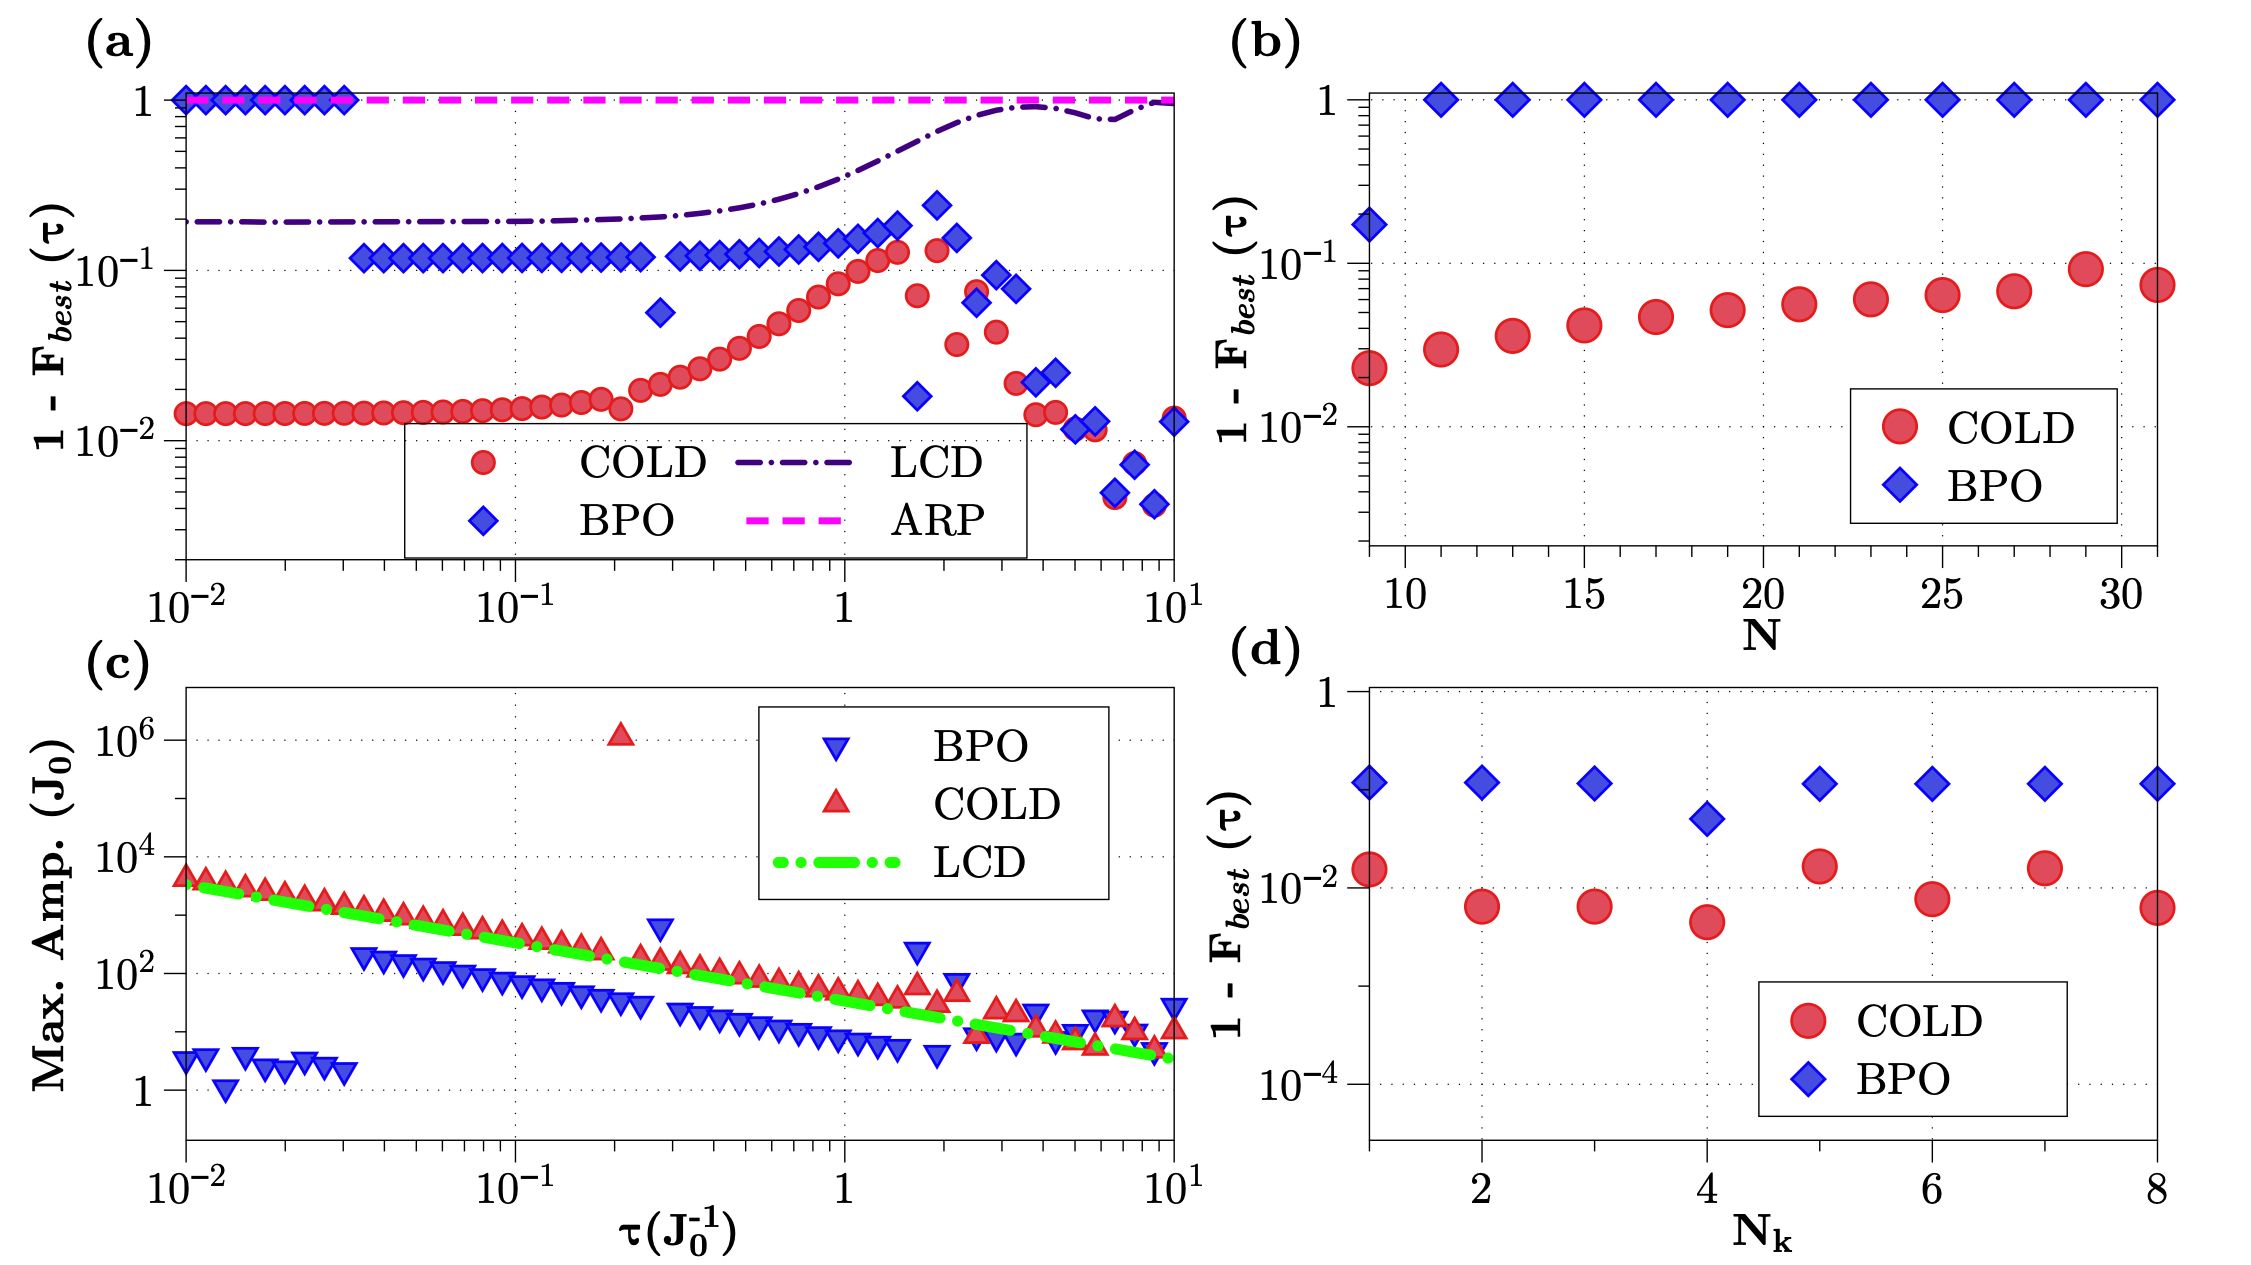
\includegraphics[width=\linewidth]{images_v1/synthetic_lattice.png} \caption[COLD plots for ARP transport in a synthetic lattice]{Optimisation of state transfer in a synthetic lattice.  In (a) we compare the fidelities obtained via the bare \acrref{ARP} protocol (pink dashed line) and \acrref{FO} \acrref{LCD} implemented in \cite{meier_counterdiabatic_2020} (purple dash-dot line) to \acrref{BPO} (blue diamonds) and \acrref{COLD} (red circles). (c) Maximum amplitude of the tunneling term at each driving time for \acrref{LCD} (green dash-dot line) as given by Eq.~\eqref{eq:tunneling} as well as \acrref{COLD} (red triangles) which includes additional control parameters (Eq.~\eqref{eq:synthetic_control_funcs}) and BPO (blue triangles) which omits the modifications due to CD but retains the control terms. In both (a) and (c) we simulate $N = 7$ lattice sites and use $N_k = 1$ parameter for optimisation of BPO and COLD.  (b) Scaling of fidelities with increasing number of lattice sites (where $N_k = 1$) for both COLD (red circles) and BPO (blue diamonds). (d) does the same for the number of parameters while keeping $N=7$.  Note that both (b) and (d) are simulated for driving time $\tau = 0.5 J^{-1}$ and the best fidelities are obtained across 500 optimisations. Figure reproduced from \cite{cepaite_cold_2023}.}\label{fig:Synthetic}
\end{figure}

In order to implement COLD we once again have to include a control component into the Hamiltonian:
\begin{equation}\label{eq:ising_control_nocrab}
    \begin{aligned}
        H_{\beta}(\hbb, \betabb, \lambda) = H_0(\hbb, \lambda) + \sum_n^N f_{\rm opt}^{N_k}(\betabb, \lambda) (c_n^{\dag}c_{n+1} + H.c.),
    \end{aligned}
\end{equation}
where the function $f_{\rm opt}^{N_k} = \sum_k^{N_k} \beta_k(\lambda)$ is the same as in Eq.~\eqref{eq:ising_chain_BPO_H}. This control pulse can be viewed as modifying the tunneling terms:
\begin{equation}\label{eq:synthetic_control_funcs}
    \begin{aligned}
        J_n(\lambda) \rightarrow J_n^{\rm opt}(\betabb, \lambda) &= J_n(\lambda) + f_{\rm opt}^{N_k}(\betabb, \lambda), \\
        \Rightarrow J_{n, \rm CD}(\betabb, \hbb, \lambda) &= \sqrt{J_n^{\rm opt}(\betabb,\hbb, \lambda)^2 + (\alpha_n(\hbb, \betabb, \lambda)/\tau)^2} \\
        \Rightarrow \phi_{n, \mathrm{CD}}(\betabb, \hbb, \lambda) &= \arctan\left(-\frac{J_n^{\rm opt}(\betabb, \lambda)\tau}{\alpha_n(\betabb, \hbb, \lambda)}\right),
    \end{aligned}
\end{equation} 
and the control functions are optimised using Powell's method as before by minimizing with respect to the fidelity of the final state, where the population has been fully transferred to the opposite lattice site. 

Now that all of our ducks are in a row, we first consider a system size of $N=7$ sites which was successfully experimentally probed in \cite{meier_counterdiabatic_2020}, where final state fidelities of $0.75$ were achieved for $\tau = 1$ms with a final tunnelling strength of $J/\hbar = 1/2\pi kHz$ (equivalent to $\tau \sim 1 J_0^{-1}$ in our units). We initially confirm the breakdown of \acrref{ARP} in this setting for fast times, and the success of the \acrref{LCD} protocol at short times, as shown in Fig.~\ref{fig:Synthetic} (a) and found in \cite{meier_counterdiabatic_2020}. Implementing \acrref{BPO} on its own manages to enhance the achievable fidelities at intermediate times of $\tau > 0.03 J^{-1}$. However, eventually, as observed in all scenarios in this work, \acrref{BPO} becomes stuck in the initial state at fast evolution times. Implementing the \acrref{COLD} protocol achieves an order of magnitude improvement in the fidelity over \acrref{LCD}. This is also plotted in Fig.~\ref{fig:Synthetic}(a).

It may be that \acrref{COLD} achieves this advantage by pumping power into the tunnelling term, as discussed in the Ising chain example, but we can see in Fig.~\ref{fig:Synthetic}(c) that the maximum amplitude of the tunnelling term tracks that of \acrref{LCD}. A key issue for experiments is the maximum amplitude achievable by a driving term and with this result we can stipulate that \acrref{COLD} is likely to be feasible in the same regimes as \acrref{LCD} in this synthetic lattice system, but with far higher resulting fidelities. There is single outlier at intermediate times as indicated by the single point peaking in maximum amplitude in Fig.~\ref{fig:Synthetic}(c), this is the exception to the rule, where the optimisation has found a marginally higher fidelity (see the corresponding point in Fig.~\ref{fig:Synthetic}(a)) by pumping in more power.

Furthermore, we explore the fidelities with increasing system size for both \acrref{BPO} and \acrref{COLD} in Fig.~\ref{fig:Synthetic}(b). While both protocols show a decreasing fidelity with increasing system size as expected, \acrref{COLD} does not suffer from getting stuck in the initial state, which is what happens in the \acrref{BPO} case as fidelities go to unity for larger systems in Fig.~\ref{fig:Synthetic}(b). This is the same mechanism as for the short driving times in Fig.~\ref{fig:Synthetic}(a). We also find, as plotted in Fig.~\ref{fig:Synthetic}(d), that increasing the number of optimisable parameters $N_k$ in the control pulse does not contribute to an improvement in the results either for \acrref{BPO} or \acrref{COLD}. This means that, at least in this very simple control setting, there is no reason to expect that \acrref{BPO} will outperform \acrref{COLD} by simply adding more complexity to the control pulse.

It is important to acknowledge once again that it may be possible to achieve better results for both the control Hamiltonian and \acrref{COLD} with the use of more sophisticated optimal control methods like \acrref{CRAB}/\acrref{COLD}-\acrref{CRAB} or a global optimiser instead of Powell's method. Any of these methods might prove to be better, but they are also far more computationally intensive and the results presented already show significant imrpovements over \acrref{LCD} or the bare Hamiltonian. In the case where such a protocol is to be implemented in practice, it would be advantageous to explore more refined control methods than those presented here.

\section{Preparing GHZ states in a system of frustrated spins}\label{sec:6.4_ghz_states}

Multipartite entanglement is a powerful resource for quantum computing and more broadly in quantum technologies, offering unique capabilities for information processing \cite{nielsen_quantum_2010}, secure communication \cite{bostrom_deterministic_2002}, high-precision measurements \cite{kim_heisenberg-limited_2022}, and understanding the foundations of quantum mechanics \cite{einstein_can_1935}. An example of such highly entangled states is the GHZ (Greenberger–Horne–Zeilinger) state \cite{greenberger_bells_1990} on $N > 1$ spins:
\begin{equation}\label{eq:GHZ_state}
    \ket{\rm GHZ} = \frac{1}{\sqrt{2}} (\ket{0}^{\otimes N} + \ket{1}^{\otimes N}),
\end{equation}
here written in the $0,1$ qubit basis.

It is possible to prepare such states in a system of frustrated spins (see Fig.~\ref{fig:ghz_mainfig}(a)) for odd $N > 1$ via an annealing protocol. The Hamiltonian describing such a system is
\begin{equation}\label{eq:ghz_hamiltonian}
    H_0(\hbb, \lambda) = J(\lambda) \Big( \sum_{j}^{N-1} \sz_j \sz_{j+1} + \sum_{j}^{N-2} \sz_j \sz_{j+2} \Big) + h(\lambda) \Big( \sum_j^N (\sz_j + \sx_j) \Big).
\end{equation}
where $\hbb = \{ J(\lambda), h(\lambda) \}$ with $\lambda = \frac{t}{\tau}$, $J(\lambda)= - J_0$ and
\begin{equation}
    h(\lambda) = - h_0 \left(1 - \sin^2\left(\frac{\pi}{2} \sin^2 \left( \frac{\pi}{2} \lambda \right) \right)\right).
\end{equation}
The parameters used for the results in this section are $J_0 = 1$ and $h_0 = 10J_0$, meaning the spins start in close to the $\ket{\downarrow^{\otimes N}}$ state. 

In this case, we will apply both \acrref{FO} \acrref{LCD} and \acrref{SO} \acrref{LCD} ans\"{a}tze. The former is the same one as used previously for the Ising chain case, Eq.~\eqref{eq:ising_fo_agp}, while the latter will consist of additional operators between next-nearest-neighbour spins to reflect the geometry of the bare Hamiltonian:
\begin{equation}\label{eq:ghz_so_lcd}
    \begin{aligned}
        \approxAGP^{(2)}(\hbb, \lambda) &= \gamma(\hbb, \lambda) \Big( \sum_{j}^{N-1} \sx_j \sy_{j+1} + \sum_{j}^{N-2} \sy_j \sx_{j+2} \Big) \\
        &+ \zeta(\hbb, \lambda) \Big( \sum_{j}^{N-1} \sz_j \sy_{j+1} + \sum_{j}^{N-2} \sy_j \sz_{j+2} \Big).
    \end{aligned}
\end{equation}
As $H_0$ is simply the Ising Hamiltonian with added couplings between spins $j$ and $j+2$, its \acrref{LCD} coefficients can be found by using the coupled equations in Appendix~\ref{app:arbitrary_ising_derivation} and setting the unused operator coefficients to $0$. 

What remains is to construct the optimal control pulse, which in this case will be done using the \acrref{GRAPE} method from Sec.~\ref{sec:3.3.2_GRAPE}. The control Hamiltonian is
\begin{equation}\label{eq:ghz_control}
    H_{\beta}(\betabb, \hbb, \lambda) = H_0(\hbb, \lambda) + f^{N_k}_{\rm GRAPE}(\betabb, \lambda) \sum_j^N \sz_j,
\end{equation}
where the pulse $f^{N_k}_{\rm GRAPE}$ is comprised of $N_k$ time slices $\Delta \lambda = \lambda_{k+1} - \lambda_k$, such that $N_k \times \Delta \lambda = 1$. During each slice $\lambda_k$, a piecewise constant control amplitude $\beta_k(\lambda_k) = c_k$, is applied to the control system, with $c_k$ denoting the optimisable parameter which represents the amplitude of the pulse in the interval $[\lambda_k, \lambda_{k+1})$. Thus, the pulse comprises of $N_k$ optimisable parameters for $N_k$ time slices. In order to enforce the constraints that the control pulse vanish at the beginning and end of the protocol and to make the pulse more smooth, we also apply a shaping function, which acts during each time interval $[\lambda_k, \lambda_{k+1})$ as
\begin{equation}
        f_{\rm shape}(\beta_k, \lambda_k) = c_k \tanh (\kappa \theta(\lambda_k)) \tanh (- \kappa \theta(\lambda_k - \tau)),
\end{equation}
with $\theta(\lambda) = \sin \frac{\pi}{2} \lambda$ and $\kappa = 30$ an offset parameter. As discussed in Sec.~\ref{sec:4.2_COLD_QOCT}, we use spline interpolation to calculate the derivatives of the control drive when they are required to obtain the \acrref{LCD} drives. The resulting function requires more parameters than the chopped basis we chose to use in previous examples, but it also allows for more flexibility in the final shape of the drive. Furthermore, due the increased number of parameters and search space, instead of Powell optimisation as in previous examples we choose to instead implement dual annealing, first presented in detail in Sec.~\ref{sec:3.1.3.3_dual_annealing}. Dual annealing is a global optimiser and while computationally more costly, is far better in the case of a complex parameter space with multiple minima, which is what may be expected in this case (see Fig.~\ref{fig:ghz_contours} later in the thesis). In this case, instead of referring to the optimised control Hamiltonian of Eq.~\eqref{eq:ghz_control} as \acrref{BPO}, we will instead dub it `bare dual-annealing' or \acrref{BDA}. 

As well as implementing the \acrref{GRAPE} pulse for all spins as in Eq.~\ref{eq:ghz_control}, as this is a more interesting and complex system than those encountered previously, we will include a separate protocol where three separate control pulses are used: one for each corner spin (see Fig.~\ref{fig:ghz_mainfig}(a)) and one for all the spins in-between. The reason for this choice of pulses is because it is often easier to independently address the edges of a lattice in practical implementations of such protocols, rather than attempting to have local control of all of the spins individually. We will include a `-C' suffix to each method in order to differentiate the corner approach from that of a global control pulse. The resulting control Hamiltonian will thus have $3 \times N_k$ optimisable parameters, which is a very large search space, making the optimisation process very computationally expensive when compared to all of the previous examples discussed in this Chapter. 

In Fig.~\ref{fig:ghz_mainfig}(c) we plot the resulting final state fidelities at different total driving times $\tau$ for a 5 spin frustrated system. We implement \acrref{BDA}, \acrref{FO} and \acrref{SO} \acrref{COLD} as well as their corner-optimised versions while optimising the pulse parameters for final state fidelity with respect to the GHZ state of Eq.~\eqref{eq:GHZ_state}. We observe that \acrref{FO} \acrref{COLD} is not particularly effective at short driving times and does not move the system out of its initial state (see the density matrix plots in (b)), regardless of whether or not separate control is applied to the corner spins. This is very likely due to the fact that the $\sy$ terms making up \acrref{FO} \acrref{LCD} are only a small contribution to the full counterdiabatic drive and thus we need to look to higher-order ans\"{a}tze to see improvements. Notably, the bare control protocol \acrref{BDA} does not fare any better, refusing to budge from the initial state at very small $\tau$. \acrref{SO} \acrref{COLD}, on the other hand, shows a five-fold improvement over the first order when a global optimisable drive is applied and up to two orders of magnitude improvement when the corner spins are driven separately at short times ($\tau = 0.001J_0^{-1}$).  We run optimisations for larger systems at time $\tau = 0.1J^{-1}$ and find that this advantage is retained even with increasing system size, as plotted in Fig.~\ref{fig:ghz_mainfig}(d). This is a large improvement over a recent result presented in \cite{sun_optimizing_2022}, where optimal control was used to directly determine \acrref{SO} \acrref{LCD} coefficients for preparing the GHZ state on an Ising chain rather than creating a control Hamiltonian. At 10 spins the final state fidelity for $\tau = 1J_0^{-1}$ obtained in their paper was 0.18, while we reach a fidelity of 0.72 for 15 spins when using corner optimisation at $\tau = 0.1J_0^{-1}$. 

\subsection{Tripartite GHZ entanglement}\label{sec:6.4.1_t3}

\begin{figure}[t!]
    \centering
    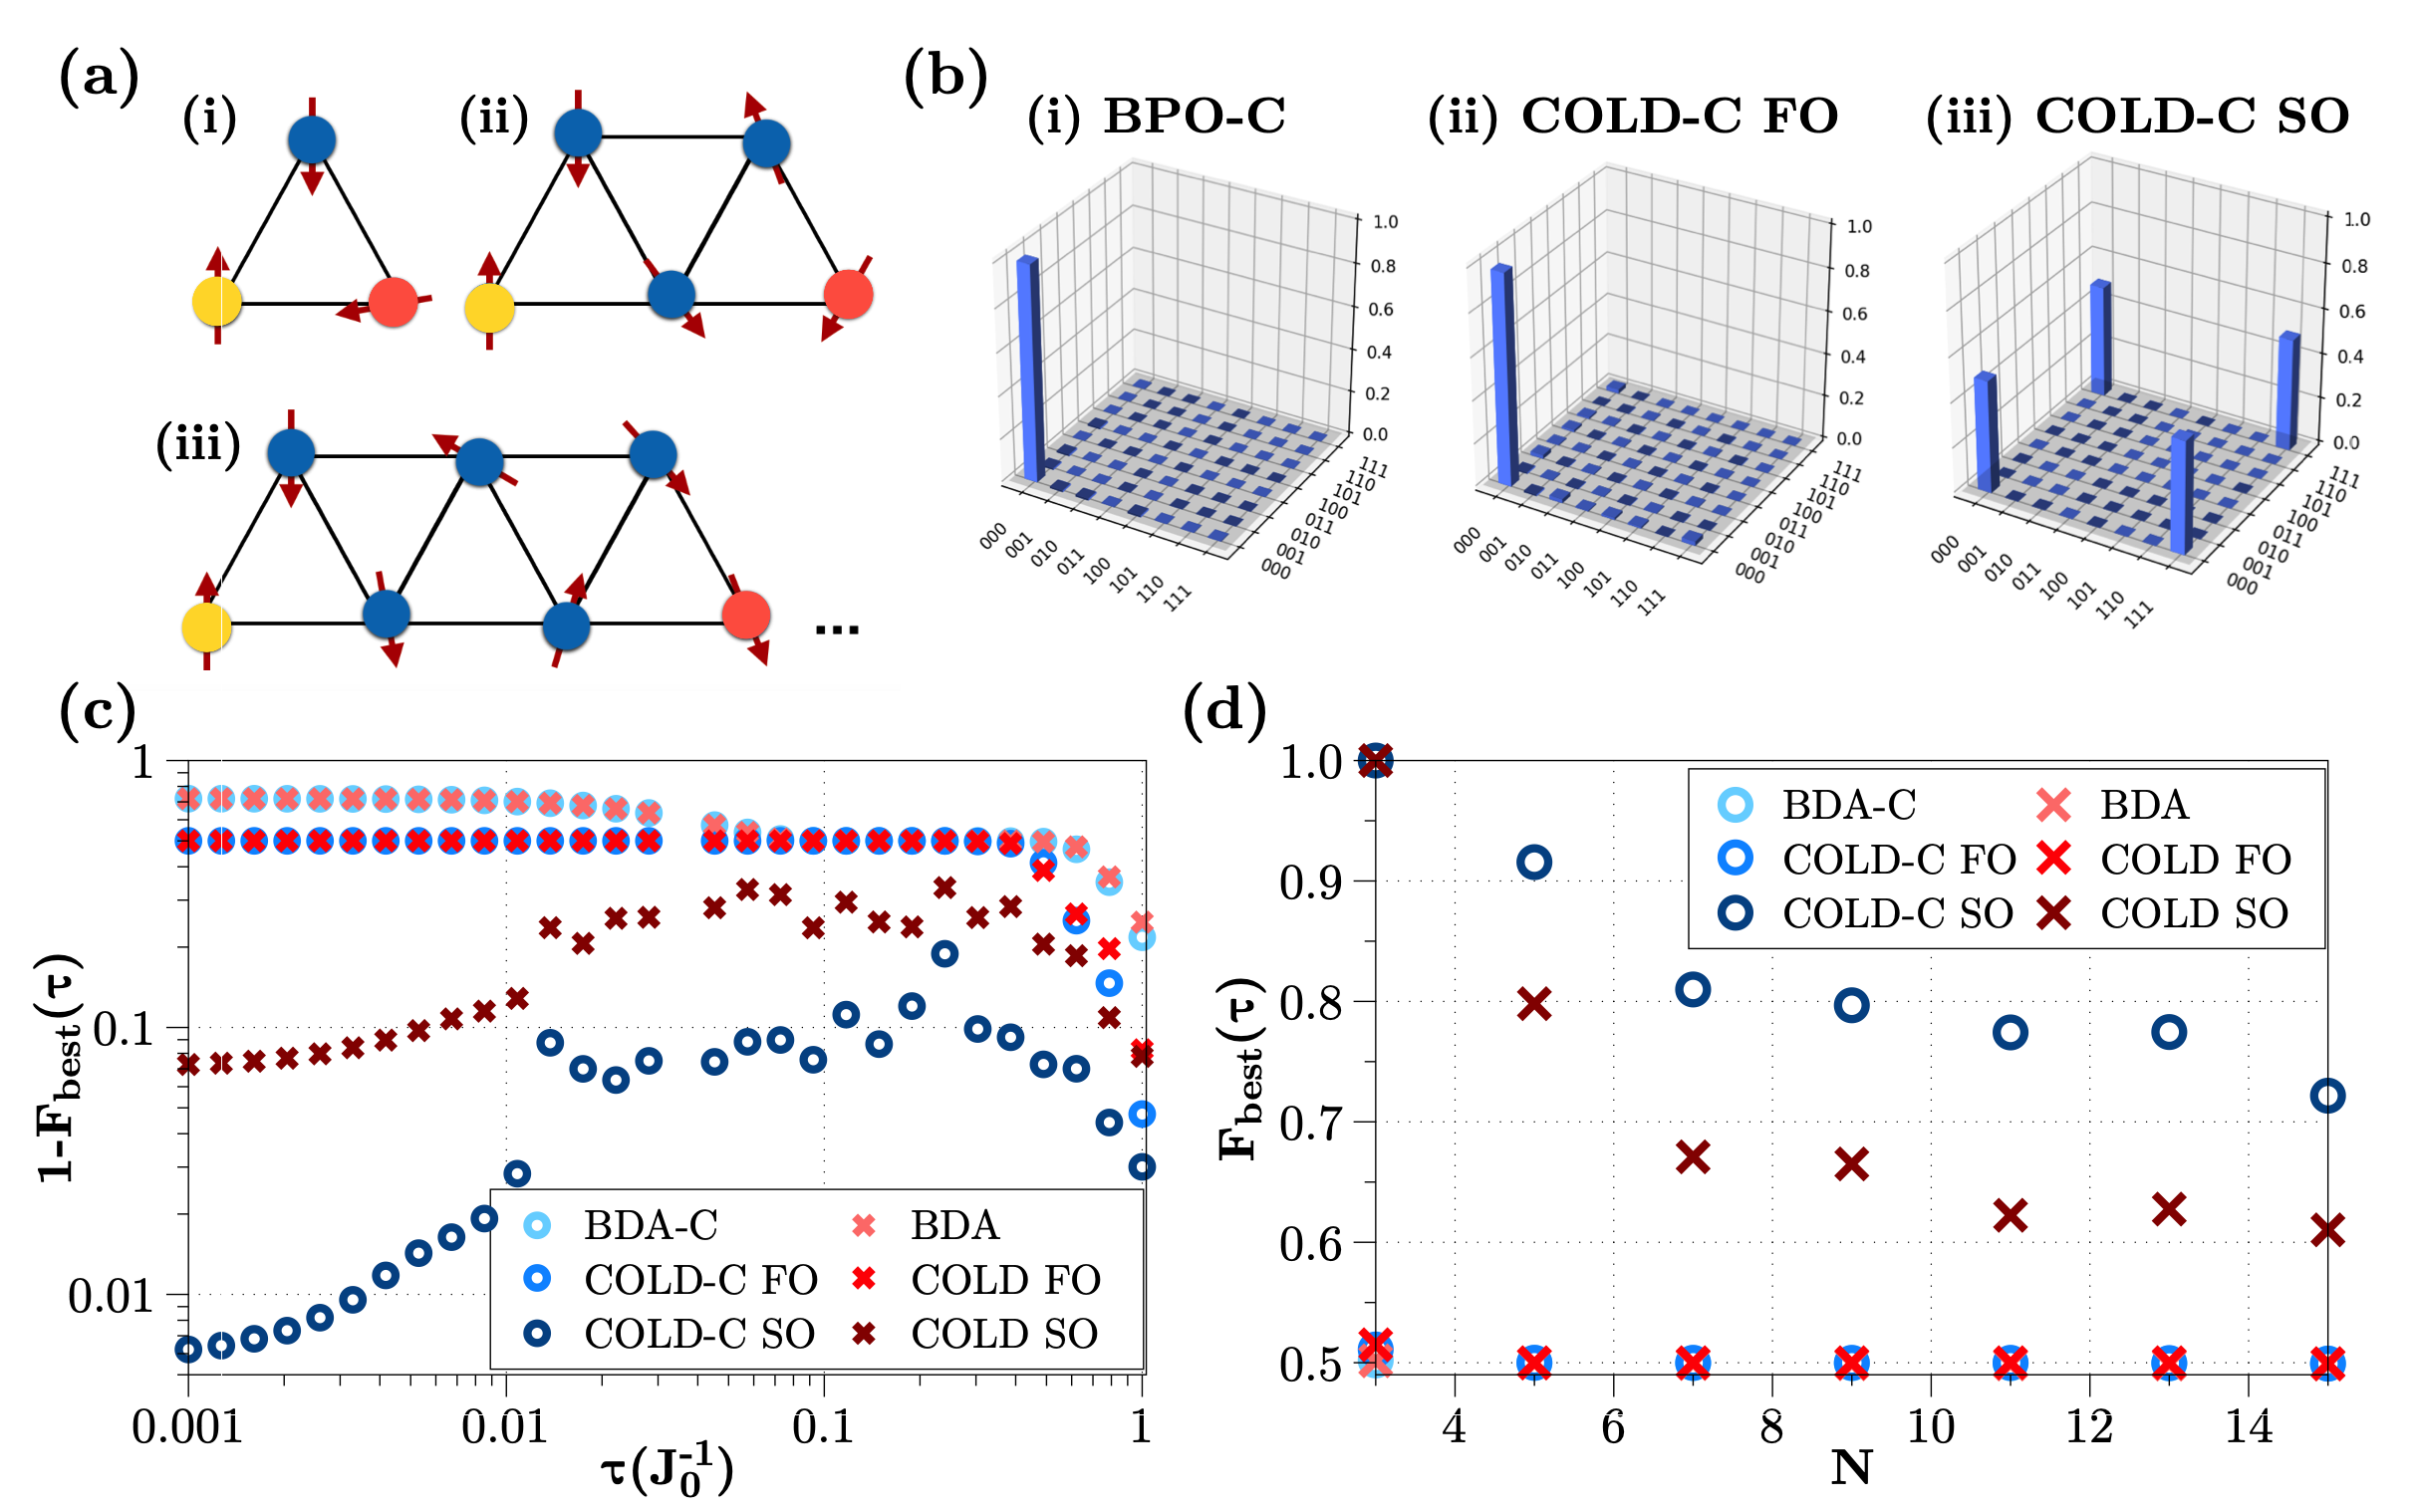
\includegraphics[width=\linewidth]{images_v1/frustrated.png} \caption[Preparation of GHZ states in a system of frustrated spins.]{GHZ state preparation in systems of frustrated spins. Spins are arranged in triangular formations as depicted in (a) for (i) 3, (ii) 5 and (iii)7 spins, with spins on the vertices and edges representing couplings.  In the case of corner optimisation, three separate optimisable drives are applied: one for the yellow corner spin, one for the red corner spin and a third drive for all of the blue spins in-between. (b) Density matrix plots of the final state of a 3 spin triangle after an evolution time $\tau = 0.1J_0^{-1}$ when optimised using (i) BDA-C, (ii) \acrref{FO} \acrref{COLD}-C and (iii) \acrref{SO} \acrref{COLD}-C. (c) Final fidelities of the GHZ state on 5 spins for optimised global drive (red crosses) and locally driven corner spins (blue rings). (d) Final fidelities at driving time $\tau = 0.1J_0^{-1}$ for different systems sizes $N$. In the global case we use $N_k = 10$ and in the corner case the total parameters are $3 \times N_k = 30$. The plots are for best results of 5 optimisations for each data point and the dual-annealing search space was bounded in the range $[-50, 50]$ for all parameters. Figure reproduced from \cite{cepaite_cold_2023}.} \label{fig:ghz_mainfig}
\end{figure}

While throughout this chapter we have focused on using final state fidelity as a cost function for the optimisation, in the case of GHZ state preparation, the goal is often the maximal entanglement of such states. Therefore, we can imagine using a cost function which maximises some entanglement metric like that in Eq.~\eqref{eq:costfunc_entanglement}, rather than the final state fidelity. This can be done in cases where several maximally entangled states are targeted, or where a single target state maximises entanglement. In the latter case, the advantage may lie in the fact that entanglement as a metric might lead to a smoother and more convex cost function landscape.

The GHZ state exhibits a particular type of entanglement: when one of the subsystems is measured, the rest are no longer entangled and collapse into a product state. This is different to the other canonical type of multipartite entanglement exhibited by the W state \cite{cabello_bells_2002}, which for 3 spins can be written as:
\begin{equation}\label{eq:W_state}
    \ket{W} = \frac{1}{\sqrt{3}}(\ket{001} + \ket{010} + \ket{100}).
\end{equation}

While measuring the entanglement of a multipartite system is not quite as simple as in the bipartite case, there exists a notion of entanglement for a system of three spins: namely, the three-tangle, first introduced in Ref.~\cite{coffman_distributed_2000}, which is maximised when a three spin system exhibits maximal GHZ-type entanglement and minimised for W-type entanglement and product states. The three-tangle is a very efficient metric and can be expressed as
\begin{equation}\label{eq:3-tangle}
	\begin{aligned}
		T_3(\ket{\psi}) &= 4 \left| d_1 - 2 d_2 + 4 d_3 \right|, \\
		d_1 &= c^2_{000}c^2_{111} + c^2_{001}c^2_{110} + c^2_{010}c^2_{101} + c^2_{011}c^2_{100}, \\
		d_2 &= c_{000}c_{001}c_{110}c_{111} + c_{000}c_{010}c_{101}c_{111} + c_{000}c_{011}c_{100}c_{111} \\
		 &+ c_{001}c_{010}c_{101}c_{110} + c_{001}c_{011}c_{100}c_{110} + c_{010}c_{011}c_{100}c_{101} \\
		d_3 &= c_{000}c_{110}c_{101}c_{011} + c_{100}c_{010}c_{001}c_{111},
	\end{aligned}
\end{equation}
where $c_{ijk}$ represents the complex coefficient of the state $\ket{ijk}$ of the three spin state $\ket{\psi}$. 

\begin{figure}[t]
    \centering
    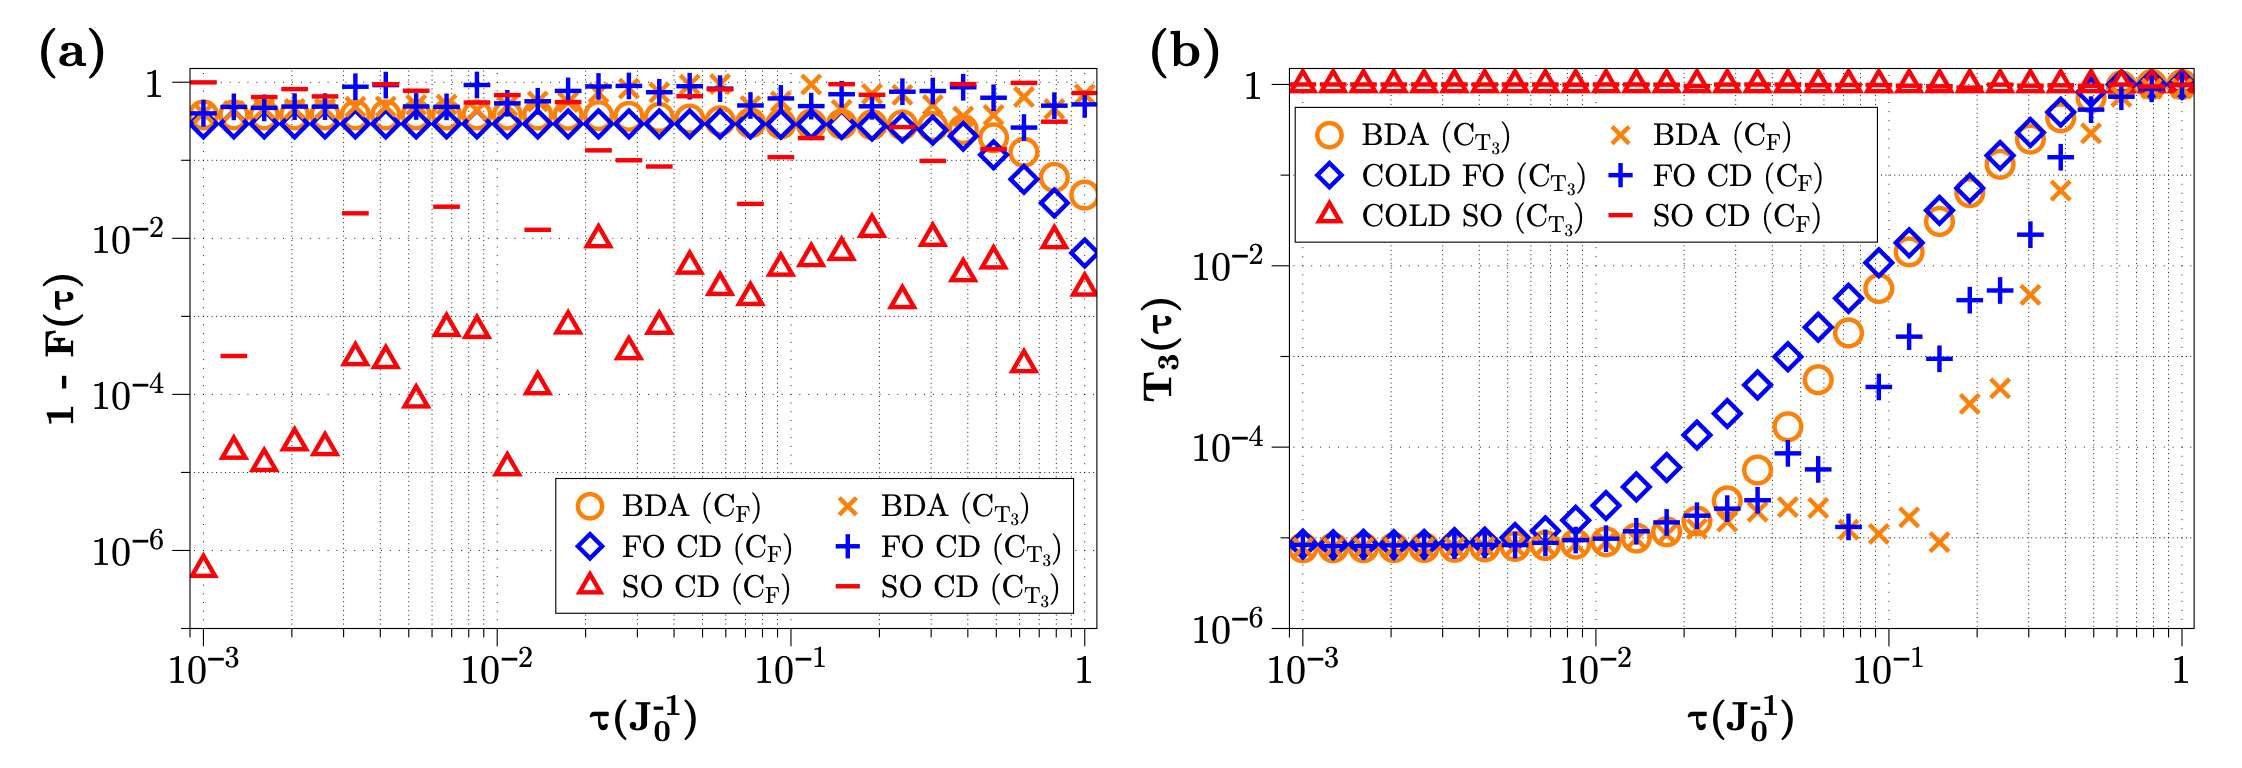
\includegraphics[width=\linewidth]{images_v1/tangle_plots.png} \caption[Preparing 3-spin GHZ states using the 3-tangle as a metric.]{Plots of $T_3$ (Eq.~\eqref{eq:3-tangle}) and fidelity $(1 - F)$ with respect to the GHZ state of the final state prepared after optimising a GRAPE pulse with $N_k = 6$ parameters for each value of $\tau$. In (a) we plot final state fidelity when optimisation is performed using $C_{\rm F}$ and $C_{T_3}$ and in (b) we plot the three-tangle from Eq.~\eqref{eq:tangle_costfunc} for the same cost functions. In both cases, the result is from a single optimisation for each data point and the dual-annealing search space bounds are $[-50,50]$ for all optimisable parameters.}\label{fig:tangle_v_fidelity}
\end{figure}

Fig.~\ref{fig:tangle_v_fidelity}(a), shows the results of the final state fidelity when optimising with $C_{\rm F}$ and optimising solely for the three tangle, using cost function
\begin{equation}\label{eq:tangle_costfunc}
    C_{T_3}(\betabb, \tau) = 1 - T_3(\ket{\psi_f(\betabb, \tau)}),
\end{equation}
where $\ket{\psi_f(\betabb, \tau)}$ is the final state obtained throughout the evolution during time $\tau$ and with optimal controls $\betabb$. In Fig.~\ref{fig:tangle_v_fidelity}(b) we investigate the values of $T_3$ obtained when using the same two cost functions. Both plots show results in a three spin system like that of Fig.~\ref{fig:ghz_mainfig}(a)(i) with only a global control pulse and dual-annealing optimisation. We find that the value of the three tangle and hence the amount of entanglement in the system begins to increase prior to any noticeable improvement in fidelity in the case of \acrref{BDA} and \acrref{FO} \acrref{COLD}, while, as expected, given the much higher fidelities obtained when using \acrref{SO} \acrref{COLD}, the entanglement is maximised for even for very small $\tau$. This is an interesting result, as it indicates that \acrref{SO} counterdiabatic operators are required to be able to speed up entanglement generation. Even when \acrref{FO} terms are applied, it long evolution times to generate entanglement. We find that even when maximising for entanglement, the results for final $T_3$ values are not very different to those obtained when optimising for final state fidelity. This is again an indication that neither \acrref{FO} terms nor the plain control Hamiltonian of Eq.~\eqref{eq:ghz_control} are enough to generate entanglement quickly and that \acrref{SO} terms are necessary for this purpose. The much lower fidelities obtained with $C_{T_3}$ are unsurprising, as the three-tangle is a measure of GHZ-type entanglement, which is maximised for several states including the orthogonal state to that presented in Eq.~\eqref{eq:GHZ_state}. This means that maximising for entanglement in this case will not always lead to final states that have high fidelity with respect to the canonical GHZ state presented at the start of this section.